%%%%%%%%%%%%%%%%%%%%%%%%%%%%%%%%%%%%%%%%%%%%%%%%%%%%%%%%%%%%%%%%%%%%%%%%%%%
%%                      Couverture report LaTeX template                 %%
%%%%%%%%%%%%%%%%%%%%%%%%%%%%%%%%%%%%%%%%%%%%%%%%%%%%%%%%%%%%%%%%%%%%%%%%%%%

\documentclass[a4paper,12pt,twoside]{article}
\usepackage{couverture}
\usepackage[T1]{fontenc}
%% \usepackage[french]{babel}
\usepackage[latin1]{inputenc}
\usepackage{url}
\usepackage{amssymb}
\usepackage{amsmath}
\usepackage{subfigure}

\usepackage{tikz}
\usetikzlibrary{arrows,positioning}

\newcommand{\couv}{{\sc Couverture}}
\renewcommand{\le}{\leqslant}
\renewcommand{\ge}{\geqslant}
\newcommand{\N}{\mathbb{N}}
\newcommand{\anysc}{\star}
\newcommand{\andthen}{\texttt{and then}}
\newcommand{\orelse}{\texttt{or else}}
\newcommand{\adaand}{\texttt{and}}
\newcommand{\adaor}{\texttt{or}}
\newcommand{\adanot}{\texttt{not}}
\newcommand{\adaif}{\texttt{if}}
\newcommand{\adathen}{\texttt{then}}
\newcommand{\adaelse}{\texttt{else}}
\newcommand{\alloyspec}[1]{\texttt{#1}}

%%%%%%%%%%%%%%%%%%%%%%%%%%%%%%%%%%%%%%%%%%%%%%%%%%%%%%%%%%%%%%%%%%%%%%%%%%%%%%

\newtheorem{theorem}{\textsc{Theorem}}
\newtheorem{definition}{\textsc{Definition}}
\newtheorem{lemma}{Lemma}[subsection]

\def\@begintheorem#1#2{\trivlist
   \item[\hskip \labelsep{#1\ #2}]\itshape}

\begin{document}
\pagestyle{empty}

\vfill

\begin{center}%
{\Large \textbf{\couv{}}}

{\Large \textbf{Technical Report on OBC/MCDC properties}}

\vfill

{\large \textbf{Abstract}}
\end{center}

This document gathers results established or formalized by the \couv{}
project team about relationships between specific coverage criteria.
%
We focus in particular on how \E{Object Branch Coverage} (OBC) relates to the
\E{Modified Condition/Decision Coverage} (MC/DC) criterion.

We provide two broad categories of results: formal proofs of important
properties over a model of the two criteria, and a machine-automated
verification of some of these properties for concrete subsets of the model
expressed in Alloy.
%
These results constitute the grounds on which our project coverage analysis
framework operates to infer source coverage results from object coverage
information out of an instrumented execution environment.

\vfill

\newpage
\pagestyle{plain}

%%%%%%%%%%%%%%%%%%%%%%%%%%%%%%%%%%%%%%%%%%%%%%%%%%%%%%%%%%%%%%%%%%%%%%%%%%%%%%

\section{Common definitions}

\subsection{Decisions, conditions}

We are considering decisions that are short circuit boolean expressions,
i.e. expressions consisting in elementary boolean conditions combined
together using only the \andthen{}, \orelse{} and \adanot{} operators.

In order to compare \E{Object Branch Coverage} to \E{Modified
Condition/Decision Coverage}, it will be shown that the appropriate
abstractions are Reduced Ordered Binary Decision Diagram. For each
decision (ROBDD), we will provide an algorithm that constructs the
associated ROBDD, whose nodes are conditions. (RO)BDDs have an entry
point, and two or more exit edges labeled True and False.

In the remainder of this document, unless otherwise indicated, all
references to BDDs denote reduced ordered BDDs. For a set S, \#S will
refer to this set's cardinal. For a decision D, cond(D) will be the
set of its conditions.

\subsection{Coverage metrics}

Coverage assessment is accomplished by exercising some piece of object
code in a variety of test cases, recording data along the way, and
then determining whether the successive executions of the object code
satisfy a given criterion of exhaustiveness. This section will define
the main coverage criterion that we will consider.

The minimum number of distinct executions required to achieve a
specific criterion is an important aspect in the evaluation of any
coverage assessment methodology. Here we establish some properties
that give a hard limit on test set size for various coverage metrics.

\subsubsection{MC/DC}

\paragraph{Formal definition:}

The formal definition of MC/DC that it used here is the one given
in~\cite{ar0118}, using a graph-coloring algorithm to determine
whether two given evaluations show the independent influence of a
condition. Amongst the various formal definitions that you may find in
the litterature, this one has the advantage to apply also to
short-circuit operators, which is mandatory in the context of \couv{}.

The following will not re-define what has already been detailed
in~\cite{ar0118}; we will just give an example on how it works and
will invit the interested reader to consult the original document. A
formal definition may also be found in the Alloy model, in file
\alloyspec{decision\_coverage.als}.

This formal definition of MC/DC uses a simple graph-coloring algorithm
to determine whether two given evaluations show the independent
influence of a condition. It first colors each node of the decision
syntax tree with both evaluations; for example, for a decision
$(A \ \andthen{} \ B) \ \orelse{} \ C$, the syntax tree can be seen
on figure~\ref{subfig:color-graph-expr}.

\begin{figure}[h]
  \centering

    \subfigure[$(A \ \andthen{} \ B) \ \orelse{} \ C$]{
      \label{subfig:color-graph-expr}

      %        or else
      %       /       \
      %   and then     C
      %  /        \
      % A          B

      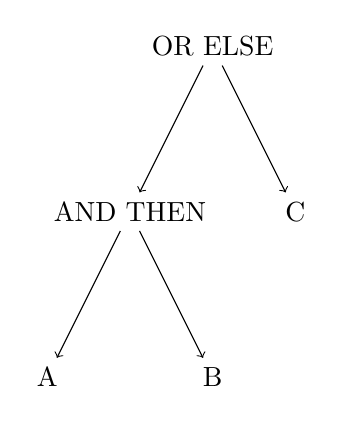
\begin{tikzpicture}[scale=1.4]
	\node (or_else) {OR ELSE}
	child[->] {
	  node (and_then) {AND THEN}
          child[->] {node (and_then_a) {A} edge from parent node[left] {}}
          child[->] {node (and_then_b) {B} edge from parent node[right] {}}
	  edge from parent node[left] {}
	}
	child[->] {node (or_else_c) {C} edge from parent node[right] {}};
      \end{tikzpicture}
    }
\end{figure}

For each evaluation, each node of the tree (atomic condition or root
of sub-decision) is colored with the value that it takes in this
evaluation: True (T), False (F), Not\_Evaluated (X).  For the
evaluation $e1 = (A = True, B = True, C = Not\_Evaluated)$, we have
the coloring given on figure~\ref{subfig:color-graph-e1}; and for $e2
= (A = False, B = Not\_Evaluated, C = False)$, we have the coloring given
on figure~\ref{subfig:color-graph-e2}.

\begin{figure}[h]
  \centering
    \subfigure[e1]{
      \label{subfig:color-graph-e1}

      %        or else T
      %       /       \
      %   and then T   C X
      %  /        \
      % A T        B T

      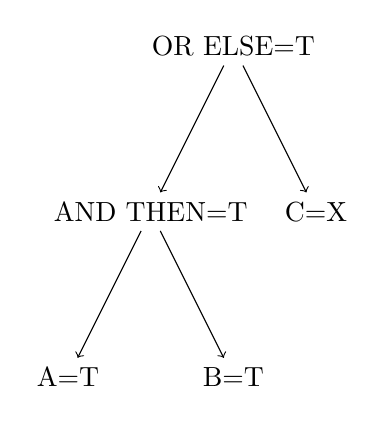
\begin{tikzpicture}[scale=1.4]
	\node (or_else) {OR ELSE=T}
	child[->] {
	  node (and_then) {AND THEN=T}
          child[->] {node (and_then_a) {A=T} edge from parent node[left] {}}
          child[->] {node (and_then_b) {B=T} edge from parent node[right] {}}
	  edge from parent node[left] {}
	}
	child[->] {node (or_else_c) {C=X} edge from parent node[right] {}};
      \end{tikzpicture}
    } \\
    \subfigure[e2]{
      \label{subfig:color-graph-e2}

      %        or else F
      %       /       \
      %   and then F   C F
      %  /        \
      % A F        B X

      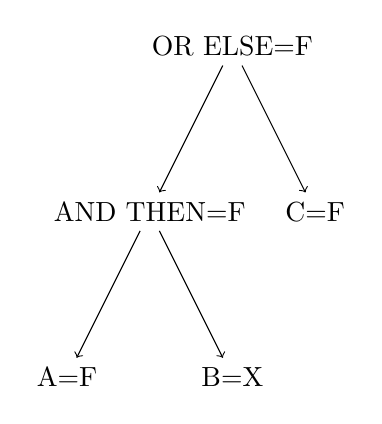
\begin{tikzpicture}[scale=1.4]
	\node (or_else) {OR ELSE=F}
	child[->] {
	  node (and_then) {AND THEN=F}
          child[->] {node (and_then_a) {A=F} edge from parent node[left] {}}
          child[->] {node (and_then_b) {B=X} edge from parent node[right] {}}
	  edge from parent node[left] {}
	}
	child[->] {node (or_else_c) {C=F} edge from parent node[right] {}};
      \end{tikzpicture}
    }
\end{figure}

Both graphs are then combined into an influence tree by xor'ing each
node. An extension of xor to three-value boolean algebra is used:
anything xor Not\_Evaluated gives False. In our case, the result is
showed on figure~\ref{subfig:color-graph-influence-tree}.

\begin{figure}[h]
  \centering
    \subfigure[Influence tree]{
      \label{subfig:color-graph-influence-tree}

      %        or else T
      %       /       \
      %   and then T   C F
      %  /        \
      % A T        B F

      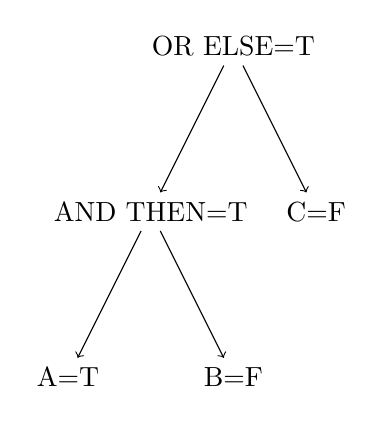
\begin{tikzpicture}[scale=1.4]
	\node (or_else) {OR ELSE=T}
	child[->] {
	  node (and_then) {AND THEN=T}
          child[->] {node (and_then_a) {A=T} edge from parent node[left] {}}
          child[->] {node (and_then_b) {B=F} edge from parent node[right] {}}
	  edge from parent node[left] {}
	}
	child[->] {node (or_else_c) {C=F} edge from parent node[right] {}};
      \end{tikzpicture}
    }
\end{figure}

The influence set of these two evaluations for the given decision is
the set of conditions that have a path of ``True nodes'' to the root.
So here, it is the singleton \{A\}.

The two classical variants of MC/DC are then defined as follow:

\begin{definition}
  \label{def:masking-mcdc}
  Given a decision D, a pair of truth vectors satisfies Masking MC/DC
  for a condition c in cond(D) if and only if its influence set is the
  singleton \{c\}.

  A test set satisfies Masking MC/DC for a decision D if, and only if,
  for each condition in cond(D), there exists a pair of tests in the
  test set that satisfies Masking MC/DC.
\end{definition}

\begin{definition}
  \label{def:unique-cause}
  Given a decision D, a pair of truth vectors satisfies Unique Cause MC/DC
  for a condition c in cond(D) if and only if its influence set is the
  singleton \{c\} and if c is the only condition that is colored with True
  in the influence tree.

  A test set satisfies Unique Cause MC/DC for a decision D if, and only if,
  for each condition in cond(D), there exists a pair of tests in the
  test set that satisfies Unique Cause MC/DC.
\end{definition}

In our example, our pair of truth vectors satisfies both Unique Cause and
Masking MC/DC for condition A.

\paragraph{Properties:}

For Unique Cause, the following property holds:

\begin{theorem}
Unique MC/DC on a decision with $n$ independent conditions is achieved with
a test set of exactly $n+1$ tests, and cannot be achieved in fewer tests.
\end{theorem}

The existence of the test set is proved by induction. For one condition,
MC/DC is achieved with two tests, one setting it True and the other False.

Now assume that the property holds for all $n \le{} N$, and consider a decision
with $N+1$ conditions. It is of the form $D = D_l \anysc{} D_r$ where
$\anysc{}$ is either \andthen{} or \orelse{}. There is also possibly a
negation, which is omitted here since it has no impact on MC/DC. For the
remainder of this proof we assume the operator is \andthen{}; the same
reasoning applies similarly for the case of \orelse{}.

$D_l$ and $D_r$ are decisions with respectively $n_l$ and $n_r$ conditions
(both at most $N$), and $n_l + n_r = N+1$. From the induction hypothesis
we have two test vector sets $T_l = \{ v_l (0) .. v_l (n_l) \}$ and
$T_r = \{ v_r (0) .. v_r (n_r) \}$ that satisfy MC/DC for $D_l$ and $D_r$
respectively, and we can arbitrarily choose the indices so that
$D_l$ is True for $v_l(0)$ and $D_r$ is True for $v_r (0)$.

We can now create a combined test set for the complete decision as follows.
$$(\forall j \in [0, n_l])\, v (j) = (v_l (j) \cdot v_r (0))$$
$$(\forall j \in [1, n_r])\, v (n_l + j) = (v_l (0) \cdot v_r (j))$$

We have thus created a set $T = \{ v(0) .. v(n_l + n_r) \}$ of $N+2$ tests.
It is immediate that the elements with indices 0 to $n_l$ give for D
the same outcome as the corresponding elements of $T_l$ for $D_l$,
and they all have identical values for the conditions coming from $D_r$,
so they show independent influence of all conditions coming from $D_l$.
Similarly the vector set $\{v(0), v(n_l+1) .. v(n_l + n_r)\}$ shows
independent influence of those conditions coming from $D_r$, so the new
test set $T$ satisfies MC/DC for $D$ and thus the induction property holds at
$N+1$ as well, since $T$ has $n_l + n_r + 1 = N+2$ elements.

The proof that this is the minimal test set size is given in~\cite{ar0118}.
As for Masking MC/DC, we have the following property:

\begin{theorem}
Masking MC/DC on a decision with $n$ independent conditions requires a
minimum of $RUTW(2*SQRT(n))$ tests, where RUTW stands for round up to
whole.
\end{theorem}

The proof of this property is given in~\cite{ar0118} as well.

The formal definitions of Masking MC/DC also allows to identify
interesting properties when only short circuit operators are used.
The following theorem tells us that, with short circuit operators,
determining Masking MC/DC is as simple as for Unique Cause, and
that no reasoning on the logical structure of the decision is needed:

\begin{theorem}
  \label{thm:masking-short-circuit}
  If a decision Dec contains only short-circuit operators, Masking MC/DC is
  reached for a condition C if and only if there exists a pair of evaluation
  (e1, e2) such that Dec[e1] = not Dec[e2], and C is the rightmost
  condition that is evaluated to True and False in e1 and e2.
\end{theorem}

The order here is the order of conditions in the decision expression; e.g.
in $(A \ \andthen{} \ B) \ \orelse{} \ C$, the order is A, B, C.

This theorem can be re-formulated in terms of influence trees, as in the
following lemma:

\begin{lemma}
  \label{lemma:short-circuit-influence-set}
  If the root node of an influence tree is colored with True, and
  if it contains only short-circuit operators, then its influence
  set contains only the rightmost True-colored condition.
\end{lemma}

This lemma can be proven by structural induction:

\begin{itemize}

\item if $D ::= C$ (simple condition decision):\\
  the root of D's influence tree is C, so if it is colored with True then
  it follows that the influence set is \{ C \}.

\item if $D ::=\ \adanot{} \ D1$, supposing that the property holds for D1:\\
  The root of D's influence tree is colored with True if and only if
  the root of D1's influence tree is colored with True as well: The
  former is evaluated to two different values (say: True, then False)
  if and only if the latter is evaluated to two different values
  (False, then True). Therefore, D1's influence set contains only the
  rightmost True-colored condition in D1's influence tree, which also
  is the rightmost True-colored condition in D's influence tree.  This
  condition is the only one to have a path of True-colored nodes to
  root in D1's influence tree, by definition of the influence set; as
  a consequence, it is also the only condition to have such path to
  root in D's influence tree. So the rightmost True-colored condition
  in D's influence tree is the only condition in its influence set.

\item if $D ::= DL \ \anysc{} \ DR$, $\anysc{}$ being a short-circuit operator,
  and supposing that the property holds for DL and DR:\\

  Let us define the boolean constant SC as follow:\\
  If $\anysc{}$ is \andthen{}, let SC be False;\\
  if $\anysc{}$ is \orelse{}, let SC be True.

  Then there are three possible evaluations for DL, DR, D:

\begin{center}
\begin{tabular}{|c|c|c||c|}
\hline
Eval name & DL            & DR            & D                    \\ \hline
e1        & \adanot{} SC  & \adanot{} SC  & \adanot{} SC         \\ \hline
e2        & \adanot{} SC  & SC            & SC                   \\ \hline
e3        & SC            & x             & SC                   \\ \hline
\end{tabular}
\end{center}

If the root of D's influence tree is colored with True, then there are only
two possible pairs of evaluations:

\begin{itemize}
\item (e1, e2): in this case, DR is colored with True and DL is colored with
False; using the induction hypothesis, we know that DR's influence tree
will have only one condition with a True-colored path to DR's root, and
consequently to D's root in D's influence tree : that will be the rightmost
True-colored condition in DR, and obviously in D. No conditions in DL
have a True-colored path to D's root, since DR's root node is colored with
False ; so the influence set contains only the rightmost True-colored
condition.
\item (e1, e3): in e3, DR is not evaluated, which means that none of its
nodes are evaluated. This means that all of them are colored with
False in DR's influence tree, and that no conditions of DR are colored
with True in D's influence tree. Thus, the rightmost True-colored condition
of D is in DL. By induction hypothesis, it is the only element of DL's
influence set; it is therefore the only condition to have a True-colored
path to DL's root node, and to D's root node. So this is the only element
in D's influence set.
\end{itemize}

\end{itemize}

The theorem has now been demonstrated in all cases. 

\subsubsection{OBC}

Applicants for DO-178 certification have sometimes proposed the use of object
code coverage instead of source code coverage as a metric to satisfy the
objectives of DO-178. The proposed approach involves measuring either
instruction coverage or branch coverage. Object instruction coverage
(OIC) requires assessing whether all object instructions are executed
at least once; object branch coverage (OBC) in addition requires that
all conditional branches be exercised for both directions (branch and
fall through). The use of object code coverage has also been proposed
as a way to cope with untraceable object code. Section 6.4.4.2 of
DO-178 indeed states: \emph{The structural coverage analysis may be
performed on the Source Code, unless the software level is A and the
compiler generates object code that is not directly traceable to Source
Code statements. Then, additional verification should be performed on
the object code to establish the correctness of such generated code
sequences}.

Untraceable object code is compiler generated machine code that impacts
the execution control flow in a way not directly visible from source code. An
example is the Ada \texttt{mod} operator, which requires an implicit
conditional branch to distinguish between positive and negative
moduli. Achieving a certain source coverage level is not indicative of
coverage of untraceable code: even a comprehensive testing campaign (from a
source coverage point of view) may not assure all object code is executed.
%
The untraceable object code is nevertheless present in the application
and may lead to unintended behaviour not verified during the testing process.

Measuring object code coverage may be a way to ensure even untraceable
code is executed during the requirement-driven testing campaign. However, CAST
paper~12~\cite{cast12} suggests the use of a \emph{traceability study} to
satisfy the additional verification activities on untraceable object code for
level~A software: a traceability study provides evidence that, in a given
context (coding standard, compiler, compilation switches), the compiler either
generates traceable code or the untraceable code is correct --- i.e. it
correctly implements the requirements expressed by the specifications of the
chosen programming language.

The issue raised by section 6.4.4.2 of DO-178, and in general the
equivalence of source and object coverage, is considered in both FAQ~42
of DO-248B~\cite{do248b} (\emph{Can structural coverage be demonstrated
by analyzing the object code instead of the source code?}) and CAST
paper~17 (\emph{Structural Coverage of Object Code}) issued by the
Federal Aviation Administration~\cite{cast17}.

Both documents assert that object code coverage can substitute for
source code coverage \emph{as long as analysis can be provided which
demonstrates that the coverage analysis conducted at the object code
will be equivalent to the same coverage analysis at the source code
level}. In the following section, we provide a precise analysis of
the conditions under which the OBC and MC/DC properties imply each
other, for a given set of test cases. It should be noted that such an
equivalence applies only in the context of a given code generator and
coding guidelines: different code generation algorithms may produce
object code whose OBC status is different for the same set of inputs
achieving a given source coverage objective.


\subsubsection{BDDBC}

As stated earlier, Binary Decision Diagrams are good abstractions to
compare the two criteria that we are considering; this section will
justify this choice. It will also introduce a new structural coverage
criterion, named \E{Binary Decision Diagram Branch Coverage}, that
relates naturally to OBC.

A Binary Decision Diagrams is a standard data structure that can be
used to represent a decision; a formal definition, along with a set of
associated algorithms and properties, can be found
in~\cite{bryant86:graphs}.  In a nutshell, BDDs can be described as a
directed acyclic graph; each node is mapped to one condition, and leaf
nodes are outcome True or False; two edges labeled True and False link
each condition to its children nodes ; those children nodes are either
a decision outcome or the next condition to evaluate, and are executed
if the father condition takes the value labeled on the corresponding
edge. Let us illustrate that on our decision
$(A \ \andthen{} \ B) \ \orelse{} \ C$; one of its BDD is shown on
figure~\ref{subfig:D1}.

One key property of BDDs is that they have a reduced form (no
isomorphic subgraph, no trivial node), and that this reduced form is
canonical (unique) for a particular decision. For instance,
figure~\ref{subfig:D1} is a reduced ordered BDD.

Now we can define BDDBC as follow:

\begin{definition}
  \label{def:bddbc}
  Given a decision D, a set of truth vectors satisfies BDDBC
  if the corresponding set of paths through its reduced ordered BDD
  covers all edges of the BDD.
\end{definition}

One can now understand how this relates to OBC. For each pair of edges that
exits from a condition node, the compiler will generate a branch that
may or may not be taken, depending on the value of the corresponding
condition; both possibilities (taking it, not taking it) maps to one
edge of the pair. If OBC is reached, then both edges should be taken,
and consequently all edges of the BDD. In other words: OBC implies
BDDBC.

This assumes that the compiler will generate one branch per condition
for each decision. In the context of \couv{}, an compilation option
-fpreserve-control-flow is provided that enforces this property; this
allows a straight-forward comparizon between OBC and BDDBC. In the
following, we specifically assume when discussing object branch
coverage of the object code, that we can instead reason, unless
indicated explicitly, on BDD branch coverage of the corresponding
(RO)BDD.


\section{Characterization of cases of BDDBC --- MC/DC equivalence}

This section discusses the distinction between expressions for which
BDDBC of the associated ROBDD implies MC/DC, and expressions for which
no such implication holds.

\subsection{Some cases of non equivalence between OBC and MC/DC}

First let us have a look at how MC/DC and object coverage relate to each
other on some simple cases. Cases of non-equivalence for decisions with up to
5 conditions have been studied in \cite{ar0720}: non-equivalence cases
have been shown to occur in decisions with three or more conditions,
and an illustration is provided with (A \andthen{} B) \orelse{} C,
where A, B and C are three independent conditions.
%
A representation of this decision's BDD is depicted on
figure~\ref{subfig:D1}.

\begin{figure}[h]
\centering

\begin{tabular}{cc}

\subfigure[]{
  \label{subfig:D1}
  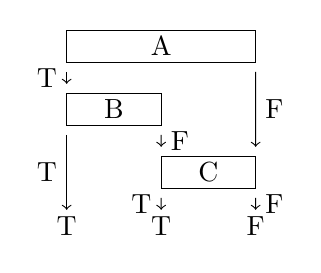
\begin{tikzpicture}[scale=0.8]

    \draw (0,0) rectangle node {A} (3,-0.5);
    \node at (0,-0.5) (if_a_true) {};
    \node at (3,-0.5) (if_a_false) {};

    \draw (0,-1) rectangle node {B} (1.5,-1.5);
    \node at (0,-1)   (b_left) {};
    \node at (1.5,-1)   (b_right) {};
    \node at (0,-1.5) (if_b_true) {};
    \node at (1.5,-1.5) (if_b_false) {};

    \draw (1.5,-2) rectangle node {C} (3,-2.5);
    \node at (1.5,-2)   (c_left) {};
    \node at (3,-2)   (c_right) {};
    \node at (1.5,-2.5) (if_c_true) {};
    \node at (3,-2.5) (if_c_false) {};

    \node at (0, -3) (outcome_true1) {};
    \node at (1.5, -3) (outcome_true2) {};
    \node at (3, -3) (outcome_false) {};

    \node at (0, -3.1) (outcome_true1_label) {T};
    \node at (1.5, -3.1) (outcome_true2_label) {T};
    \node at (3, -3.1) (outcome_false_label) {F};

    \draw [->] (if_a_true)  -- node[left] {T} (b_left);
    \draw [->] (if_a_false) -- node[right] {F} (c_right);

    \draw [->] (if_b_true)  -- node[left] {T} (outcome_true1);
    \draw [->] (if_b_false) -- node[right] {F} (c_left);

    \draw [->] (if_c_true)  -- node[left] {T} (outcome_true2);
    \draw [->] (if_c_false) -- node[right] {F} (outcome_false);

  \end{tikzpicture}
} & \subfigure[]{
  \label{subfig:D2}
  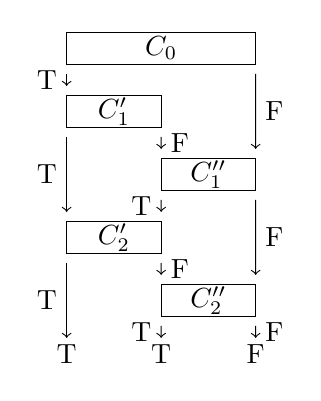
\begin{tikzpicture}[scale=0.8]

    \draw (0,0) rectangle node {$C_{0}$} (3,-0.5);
    \node at (0,-0.5) (if_c0_true) {};
    \node at (3,-0.5) (if_c0_false) {};

    \draw (0,-1) rectangle node {$C'_{1}$} (1.5,-1.5);
    \node at (0,-1)   (c1a_left) {};
    \node at (1.5,-1)   (c1a_right) {};
    \node at (0,-1.5) (if_c1a_true) {};
    \node at (1.5,-1.5) (if_c1a_false) {};

    \draw (1.5,-2) rectangle node {$C''_{1}$} (3,-2.5);
    \node at (1.5,-2)   (c1b_left) {};
    \node at (3,-2)   (c1b_right) {};
    \node at (1.5,-2.5) (if_c1b_true) {};
    \node at (3,-2.5) (if_c1b_false) {};

    \draw (0,-3) rectangle node {$C'_{2}$} (1.5,-3.5);
    \node at (0,-3)   (c2a_left) {};
    \node at (1.5,-3)   (c2a_right) {};
    \node at (0,-3.5) (if_c2a_true) {};
    \node at (1.5,-3.5) (if_c2a_false) {};

    \draw (1.5,-4) rectangle node {$C''_{2}$} (3,-4.5);
    \node at (1.5,-4)   (c2b_left) {};
    \node at (3,-4)   (c2b_right) {};
    \node at (1.5,-4.5) (if_c2b_true) {};
    \node at (3,-4.5) (if_c2b_false) {};

    \node at (0, -5) (outcome_true1) {};
    \node at (1.5, -5) (outcome_true2) {};
    \node at (3, -5) (outcome_false) {};

    \node at (0, -5.1) (outcome_true1_label) {T};
    \node at (1.5, -5.1) (outcome_true2_label) {T};
    \node at (3, -5.1) (outcome_false_label) {F};

    \draw [->] (if_c0_true)  -- node[left] {T} (c1a_left);
    \draw [->] (if_c0_false) -- node[right] {F} (c1b_right);

    \draw [->] (if_c1a_true)  -- node[left] {T} (c2a_left);
    \draw [->] (if_c1a_false) -- node[right] {F} (c1b_left);

    \draw [->] (if_c1b_true)  -- node[left] {T} (c2a_right);
    \draw [->] (if_c1b_false) -- node[right] {F} (c2b_right);

    \draw [->] (if_c2a_true)  -- node[left] {T} (outcome_true1);
    \draw [->] (if_c2a_false) -- node[right] {F} (c2b_left);

    \draw [->] (if_c2b_true)  -- node[left] {T} (outcome_true2);
    \draw [->] (if_c2b_false) -- node[right] {F} (outcome_false);

  \end{tikzpicture}
}\\
\end{tabular}

\caption{Example decision BDDs}
\label{fig:examples}
\end{figure}

From this representation, we can see that a set of three evaluations can
achieve branch coverage of the whole BDD, corresponding to the three vertical
paths in figure~\ref{subfig:D1}.
%
These evaluations are:

\begin{center}
\begin{tabular}{|c|c|c||c|}
\hline
A & B & C & (A \andthen{} B) \orelse{} C \\ \hline
T & T & x & T \\ \hline
T & F & T & T \\ \hline
F & x & F & F \\ \hline
\end{tabular}
\end{center}

where ``x'' means not evaluated and thus can be indifferently True or False.
%
Now, indeed, even though all the BDD edges are covered, MC/DC is not
met. In particular, the independent effect of conditions B on the
decision is not shown in the case of Masking MC/DC, and the
independent effect of both B and C are not shown in the case of Unique
Cause.  Since $n+1$ tests are needed to cover a decision with $n$
conditions with respect to Unique Cause MC/DC, 3 evaluations cannot cover a
three-condition decision. Masking MC/DC requires a minimum of 4 evaluations
as well in this particular case.

It turns out that this particular case can be generalized in a
quite spectacular counterexample: there exists classes of decisions
with an arbitrary high number of conditions that can be branch covered
by just three evaluations; the previous example was one element of this
class with 3 conditions.

Consider the following set $\{D_{n}\}_{n \in \N}$  of decisions:

\begin{itemize}
\item let $D_{0}$ be a simple condition decision; by convention,
      we will call $C_{0}$ its condition;
\item let us define $D_{n}$, for any $n>0$, as follows:\\
      $D_{n} = (D_{n-1} \ \andthen{} \ C'_{n}) \ \orelse{} \ C''_{n}$\\
      $C'_{n}$ and $C''_{n}$ being independent from each other and from
      any condition in $D_{n-1}$.
\end{itemize}

In other words:
\begin{itemize}
\item $D_{0} = C_{0}$
\item $D_{1} = (C_{0} \ \andthen{} \ C'_{1}) \ \orelse{} \ C''_{1}$
\item $D_{2} = (((C_{0} \ \andthen{} \ C'_{1}) \ \orelse{} \ C''_{1})\\
                 \andthen{} \ C'_{2}) \ \orelse{} \ C''_{2}$
\item $D_{3} = (((((C_{0} \ \andthen{} \ C'_{1}) \ \orelse{} \ C''_{1})\\
                 \andthen{} \ C'_{2}) \ \orelse{} \ C''_{2})\\
                   \andthen{} \ C'_{3}) \ \orelse{} \ C''_{3}$
\item ...
\end{itemize}

Figure~\ref{subfig:D2} shows the BDD for $D_{2}$, where it is visible
that all the edges can be covered by three evaluation paths which only
demonstrate the independent effect of $C_{0}$:

\begin{center}
\begin{tabular}{|c|c|c|c|c||c|}
\hline
$C_{0}$   & $C'_{1}$   & $C''_{1}$   & $C'_{2}$   & $C''_{2}$   & $D_{2}$ \\ \hline
T      & T       & x        & T       & x        & T     \\ \hline
T      & F       & T        & F       & T        & T     \\ \hline
F      & x       & F        & x       & F        & F     \\ \hline
\end{tabular}
\end{center}

We can thus build a decision $D_{n}$ with an arbitrary number of
conditions, that can be BDD branch covered by just three evaluation
paths. As Unique Cause MC/DC can only be achieved with a minimal
number of $n+1$ evaluations, and Masking MC/DC with a minimal number
of $RUTW(2*SQRT(N))$ tests, this is a striking case where BDD branch
coverage (and consequently OBC) is far from being equivalent to MC/DC.

We can now adopt a more general perspective and characterize more
precisely the difference between these two criteria.

\subsection{Construction of the ROBDD}

The BDD we associate with a decision is constructed using the following
recursive procedure:

\begin{description}
\item[Build\_BDD.Condition]
  The BDD for a decision consisting in a single condition C has the node
  "test C" as its entry point, the label True is assigned to the branch
  corresponding to "C is True", and the label False is assigned to the
  branch corresponding to "C is False".

\item[Build\_BDD.NOT]
  The BDD for $\adanot{} (D)$ is the BDD for D where the labels of the exit
  edges have been swapped.

\item[Build\_BDD.Short\_Circuit\_Operator]
  This rule defines how the BDD for $(DL) \anysc{} (DR)$ is constructed for
  any short-circuit operator $\anysc{}$.

  If $\anysc{}$ is \andthen{}, let SC be False;\\
  if $\anysc{}$ is \orelse{}, let SC be True.

  Let BL be the BDD for DL, and BR the BDD for DR.

  Then B, the BDD for D is obtained by combining BL and BR as follows:
  \begin{itemize}
    \item the entry point is that of BL
    \item the exit edge labeled SC of BL is an exit edge labeled SC of B
    \item the other exit edge of BL connects to the entry point of BR
    \item the exit edges of BR are exit edges of B with the same labels
  \end{itemize}
\end{description}

The following invariants of ROBDDs follow from the construction process:
\begin{itemize}
  \item There is exactly one BDD node for each condition.
  \item All condition nodes are reachable (i.e. there is a path from
        the entry point to any node in the BDD).
  \item There are no cycles in the BDD.
  \item Both outcomes are reachable (i.e. there is a path from the entry point
        to an exit edge labeled True and to an exit edge labeled False).
\end{itemize}

This algorithm is formally described in Alloy, in \alloyspec{build\_bdd.als}.
Given a decision D, we will now call BDD(D) its (RO)BDD as built by this
recursive procedure.

\subsection{Node ordering}

For a decision D and a condition C in D, let us call index(D,C) the
positive number built by the following recursive procedure:

\begin{description}
\item[Build\_BDD\_Order.Condition]
  The sub-decision is a single condition decision, it is of the form:\\
  $D ::= C$\\
  then index(D,C) = 1\\

\item[Build\_BDD\_Order.NOT]
  The sub-decision is of the form:\\
  $D ::= \adanot{} \ D1$\\
  then for each condition C in D, index(D,C) = index(D1,C)\\

\item[Build\_BDD\_Order.Short\_Circuit\_Operator]
  The sub-decision is of the form:\\
  $D ::= DL \ \anysc{}\ DR$\\
  then, for each condition C in D:\\
  \begin{itemize}
    \item if C is in DL, $index(D,C) = index(DL,C)$
    \item if C is in DR, $index(D,C) = index(DR,C) + \#cond(DL)$
  \end{itemize}
\end{description}

This builds a total order over the conditions of a decision; it is a
general result for such a reduced order BDD that the reflexive transitive
closure defines a total order over its nodes; this order is the same
as the one we just defined. It can also be demonstrated easily, by
structural induction, that this order is the order of conditions in
the decision's expression.

For a decision D, we will call $root(D)$ and $root(BDD(D))$ the unique
node with index 1.  This node is indeed the root node of the BDD.

\subsection{Evaluation of a decision}

Given the transformation of a decision into its ROBDD, evaluating the
decision consists in computing its value using the following BDD traversal
procedure:

\begin{description}
\item[Eval.Condition]
  The value of a decision that consists in a lone condition is the
  value of the condition.

\item[Eval.Not]
  To evaluate $\adanot{} (D)$, evaluate D and take the opposite value

\item[Eval.Short\_Circuit\_Operator]
  To evaluate $(D1) \anysc{} (D2)$, evaluate D1. If $D1 = SC$ then the
  value is SC, else evaluate D2, and the value is that of D2.
\end{description}

This algorithm is modeled in \alloyspec{decision\_evaluations.als}
The following property holds:

\begin{description}
\item[Evals\_Are\_Paths]
  Evaluating a decision is equivalent to traversing the BDD, evaluating
  each condition as BDD nodes are traversed, and using the label of the
  exit edge as the value of the decision.
\end{description}

This property, and most properties that we'll discuss here, is proved
by induction on the structure of the decision.  For each case of the
BDD\_Build procedure (Build\_BDD.Condition, Build\_BDD.Not,
Build\_BDD.Short\_Circuit\_Operator), we will assume that the the
property holds for the parameters and prove that the build step
preserves the property. A formal model for this proof can be found
in \alloyspec{bdd\_dec\_evaluations.als}.

Note that the practical implementation of coverage analysis systems based
on control flow traces relies on the assumption that the code generator
used to produce executable code from expressions actually implements this
evaluation strategy.

\subsection{Equivalence case}

We now consider the case of an expression whose BDD has no diamond paths,
i.e. for each BDD node there is exactly one path from the entry point to
that node. The following property holds:

\begin{description}
\item[BDDBC\_No\_Diamond\_Indep\_Implies\_MCDC]
  For a BDD with no diamonds, if conditions are independent, then
  BDD branch coverage implies Unique Cause MC/DC and Masking MC/DC.
\end{description}

Let's consider a condition C. Since we have BDD branch coverage,
all possible paths starting at C have been taken (by recurrence on path
length, taking advantage of no cycles and no diamonds).

From the independent outcome reachability property, we have two paths
starting at C, beginning each with one edge from C, and ending on the
two outcomes of the decision. Let's call them PCT and PCF.

These paths are disjoint: any condition appearing in one is not evaluated
in the other (because of no-diamond).

These two paths are parts of paths PT and PF from the BDD entry point to
either outcome, and they cannot differ on the part of the path from the
entry point to C.

So, PT and PF differ in C, in no other condition before C, and in no
other non-masked condition after C, so they prove independent influence
of C over the decision.

This holds for each condition in the decision, so Unique Cause MC/DC
is proved; and since Unique Cause is stronger than Masking MC/DC,
Masking MC/DC is proved as well.

This property and the non-equivalence case that follows is modeled
in \alloyspec{bdd\_coverage.als}.

\subsection{Non-equivalence case}

The general idea of this proof is to show that, for any BDD with a
diamond, we can build a set of evaluations that covers the BDD
branches in such a way that there is at least one condition for which
MC/DC is not met.

If we want to have a proof that will work for any definition of MC/DC,
we cannot rely on a failure of the independence criteria; \textit{to
independently affect} means something different in Unique Cause MC/DC
or in Masking MC/DC. So we should rather rely, if it is possible, on
the set of properties that these criteria have in common; a sort of
\textit{greatest common divisor} of the two criteria. Let us define
this Weak MC/DC criteria as follow:

\begin{itemize}
\item every possible outcome of the decision has been tried;
\item each condition in the decision has taken on every possible outcome;
\item each condition in the decision is shown to affect the outcome of the
      decision.
\end{itemize}

The only difference with MC/DC here is that Weak MC/DC does not care
if the condition \textit{independently} affects the outcome of the decision;
whatever \textit{independently} means. Weak MC/DC is weaker than any other
MC/DC criteria. So, if a set of evaluations does not satisfy Weak MC/DC,
it won't satisfy Unique Cause MC/DC or Masking MC/DC.

The formal definition would be:

\begin{definition}
  \label{def:weak-mcdc}
  Given a decision D, a pair of truth vectors satisfies Weak MC/DC for
  a condition c if and only if, in their influence tree, the node c
  and the root node are both colored in True.

  A test set satisfies Weak MC/DC for a decision D if, and only if,
  for each condition in cond(D), there exists a pair of tests in the
  test set that satisfies Weak MC/DC.
\end{definition}

It turns out that we can build a set of evaluations such that BDDBC is
reached, but not MC/DC, when the BDD has a diamond.  Let's take the
canonical example:\\
$(A \ \andthen{} \ B) \orelse{} \ C$\\
and these evaluations:

\begin{center}
\begin{tabular}{|c|c|c||c|}
\hline
A & B & C & (A \andthen{} B) \orelse{} C \\ \hline
T & T & x & T \\ \hline
T & F & T & T \\ \hline
F & x & F & F \\ \hline
\end{tabular}
\end{center}

This set covers this decision for BDDBC. However, this does not meet
Weak MC/DC; whenever B is evaluated, the decision outcome is True. So
this cannot show that B affects the outcome of the decision.

Let us give a general idea of how we would prove that in the general
case. First, remember that we are dealing with reduced ordered BDDs;
so each node can be ordered. This property allows us to have a
proper concept of ``last diamond node'' and its ``last parent''. In our
example, the last diamond node would be C, its last parent B.

Now, we would show that the last parent of the last diamond node has
an interesting property: one of its exit edge is always connected
directly to an outcome (for B, it is outcome True). Its other exit
edge being connected to the last diamond node (obviously), it is
possible to cover this edge in such a way that the outcome of the
corresponding evaluation is the same as the ``direct outcome'';
e.g. when evaluating B to False, we would evaluate C to True and exit
on True. We know that this is possible using the property that, from
each node of the BDD (and, in this case, the diamond C), there exists
at least one evaluation that reaches outcome True and at least one that
reach outcome False.

This means that we can cover all exit and incoming edges of the last
parent of the last diamond in such a way that the evaluations \textit{always}
exit on the same outcome; and, from the property of its exit edges, we
can see that this set of evaluations can be completed to reach BDDBC
\textit{without evaluating this node anymore}. This builds a BDD coverage
that does not satisfy Weak MC/DC for this node.

The following sections will detail this proof.

\subsubsection{Last diamond}

We have previously built a function index(D,C) that defines a full
order over the nodes of a (RO)BDD. Based on this function, we can
define the following entities:
\begin{itemize}
\item in a BDD, let the last node be the node with the greatest index;
\item let a diamond node be a node with more than one parent;
\item let the last diamond node of a decision be the diamond with the
      greatest index;
\item let the last parent of a node be the parent with the greatest index.
\end{itemize}

Some examples from our canonical case
$D ::= (A \ \andthen{} \ B) \orelse{} \ C$:
\begin{itemize}
\item index(D,A) = 1, index(D,B) = 2, index(D,C) = 3;
\item the last diamond node is C; it is also the last node;
\item the last parent of C is B.
\end{itemize}

We have the following properties:

\begin{lemma}
  \label{lemma:last-node}
  The two exit edges of the last node are connected to both outcomes.
\end{lemma}

\begin{lemma}
  \label{lemma:last-parent-of-the-last-diamond}
   If a BDD contains diamonds, then the last parent of the last diamond
   has an exit edge that is directly connected to an outcome.

   This outcome will be called the direct outcome (of the last of parent of
   the last diamond). The edge connected to the the direct outcome will be
   called the direct exit edge.
\end{lemma}

This can be seen in our example:
\begin{itemize}
\item the last node being C, its exit edges are connected directly to True and
      False;
\item the last parent of the last diamond being B; when it is True, the outcome
      True is reached.
\end{itemize}

The two properties can be proved by structural induction on the BDD.
The first is the easiest one and we will keep it as an exercise for the
reader. Here is a proof of the second one:

\begin{itemize}
\item if $D ::= C$ (simple condition decision):\\
  the BDD does not contain any diamonds, so the property is trivially true
  in this case.

\item if $D ::=\ \adanot{} \ D1$:\\
  if D1 does not contain diamond, D does not either, the propery is trivial
  as well. If it does contain diamond, well, only outcome labels are different
  between BDD(D) and BDD(D1), so the property holds for D if it holds for D1.

\item if $D ::= DL \ \anysc{} \ DR$, supposing that the property holds
  for DL and DR; four cases then:

  \begin{itemize}
  \item If no diamonds were in BDD(DL) and BDD(DR), and none were introduced
    by building BDD(D) from them: then BDD(D) contains no diamonds, the
    property is trivial.

  \item If DR contains a diamond: then the last diamond node of D is
    the last diamond node in DR. By construction, BDD(DR) is a
    sub-tree of BDD(D), the exit edges of the last diamond node are
    the same in BDD(DR) and in BDD(D). So if the property holds for
    DR, it holds for D.

  \item If DR contains no diamonds, and if building BDD(D) from
    BDD(DR) and BDD(DL) introduces a new diamond: this new diamond
    node has to be root(DR), as only this node has gained new incoming
    edges: in Build\_BDD, the exit edges of BDD(DR) labeled ``not SC''
    are connected to BDD(DL)'s root. Therefore, its parent nodes are
    all in cond(DL). And the last node of BDD(DL) is one of these
    parent nodes; by property~\ref{lemma:last-node}, it has an exit
    edge to ``not SC'' in BDD(DL). Its other exit edge will remain
    unchanged in BDD(D) and will be connected to an outcome
    (``SC''). This last node of BDD(DL) is also the last parent of
    this diamond node, as no other nodes in cond(DL) have a greater
    index. And (finally), this introduced diamond node is D's last
    diamond node, as DR contains no diamonds (initial hypothesis). So
    we have identified the last parent of the last diamond and showed
    that one of its exit edges is connected to an outcome in BDD(D); that's
    the property that we were trying to prove.

  \item If DR contains no diamonds, and if no diamonds were introduced
    when building BDD(D), but if DL contains a diamond: the last
    diamond node in D is the same node as the last diamond node in DL.
    The last parent of the last diamond in DL has an exit edge that
    connects to SC; otherwise, it would be connected to BDD(DR)'s root
    when building BDD(D), and as the last node would also be connected
    to this root node (it also has an exit edge to SC in DR, as a
    consequence of property~\ref{lemma:last-node}), BDD(DR)'s root
    would have at least two fathers in D, which contradicts the
    hypothesis that no diamonds were introduced. So this exit edges of
    the last parent of the last diamond in DL (and D) will still be
    connected to an outcome after building D. So the property is true
    in this case as well.
  \end{itemize}
\end{itemize}

The property~\ref{lemma:last-parent-of-the-last-diamond} has now been
established in all possible cases. This proof will actually be quite
useful as its structure will be used to build a coverage that satisfies
BDDBC but not Weak MC/DC.

\subsubsection{Path though BDDs - Conventions}

Some conventions first to help us manipulate paths through BDD:

\begin{itemize}
\item For two paths pl, pr into two different BDDs,
  concat(pl, pr) is the concatenation of these two paths obtained by replacing
  the outcome of pl by the first node in pr.

\item For two set of paths PL, PR through two different BDDs, merge(PL, PR)
  is the set built by doing an arbitrary mapping of each element
  of PL to each element of PR, and concatenating each pair; as these
  two sets may not have the same number of elements, all the remaining
  elements of the greatest set will be mapped to one arbitrary element
  of the smallest set.

\item For any set of paths PS through a BDD (each going from the root node to
  an outcome), let us call path\_to(True, PS) the subset of paths reaching
  outcome True, and path\_to(False, PS) the subset reaching False. We have
  the obvious property:

  $PS = path\_to(True, PS) + path\_to(False, PS)$
\end{itemize}

\subsubsection{Building a BDD branch coverage that does not verify Weak MC/DC}

For a given decision D, our coverage will be ensured by the union of
three sets of paths Short\_Circuit\_LPLD(D), Long\_Circuit\_LPLD(D) and
LPLD\_Not\_Evaluated(D), which verifies the following set-specific
invariants:

\begin{description}
\item[Short\_Circuit\_LPLD\_Invariant]
  If BDD(D) is diamondless, Short\_Circuit\_LPLD(D) is empty;
  otherwise, it contains a non-empty set of paths, each reaching the
  last parent of the last diamond node and then exiting on its direct
  outcome.

\item[Long\_Circuit\_LPLD\_Invariant]
  If BDD(D) is diamondless, Long\_Circuit\_LPLD(D) is empty;
  otherwise, it contains a non-empty set of paths, each reaching the last
  parent of the last diamond node, then going to the last diamond node, and
  then reaching the same outcome as Short\_Circuit\_LPLD(D).

\item[LPLD\_Not\_Evaluated\_Invariant]
  No path in LPLD\_Not\_Evaluated(D) evaluates the last parent of the last
  diamond node.
\end{description}

...plus one other ``global'' invariants:

\begin{description}
\item[BDDBC\_Coverage\_Invariant]
 The union of these three sets covers each edges of the considered
 BDD.
\end{description}

As a consequence of this last invariant, we will now call
BDDBC\_Coverage the union of these three sets:

\begin{align*}
  BDDBC\_Coverage(D) & = Short\_Circuit\_LPLD(D)\\
                     & + Long\_Circuit\_LPLD(D)\\
                     & + LPLD\_Not\_Evaluated(D)
\end{align*}

Note also that an other property falls naturally from
LPLD\_Not\_Evaluated\_Invariant and BDDBC\_Coverage\_Invariant:

\begin{description}
\item[Incoming\_Edges]
  The union of Long\_Circuit\_LPLD and Short\_Circuit\_LPLD covers all incoming
  edges of the last parent of the last diamond node.
\end{description}

Anyway, here is the definition, case by case, of a recursive build
procedure that builds such sets from a decision D. As always when
doing a structural induction, it assumes that all its sub-decisions
have such sets verifying these invariants (not considering D as a
sub-decision of D, obviously; ``strict'' sub-decisions):

\begin{description}
\item[Build\_BDD\_Cov.Condition]
  The sub-decision is a single condition decision, it is of the form:\\
  $D ::= C$\\
  In this case:
  \begin{align*}
    Short\_Circuit\_LPLD(D) & = Long\_Circuit\_LPLD(D) = \{\}\\
    LPLD\_Not\_Evaluated(D) & = \{C -> True, C -> False\}\\
  \end{align*}


\item[Build\_BDD\_Cov.NOT]
  The sub-decision is of the form:\\
  $D ::=\ \adanot{} \ D1$

  Then Short\_Circuit\_LPLD(D) is built by switching the outcome of each
  path contained in Short\_Circuit\_LPLD(D1). Same operations for
  Long\_Circuit\_LPLD(D) and No\_LPLD(D).


\item[Build\_BDD\_Cov.Short\_Circuit\_Operator]
  The sub-decision is of the form:\\
  $D ::= DL \anysc{} DR$

  Four sub-cases:

  \begin{itemize}
  \item No diamonds:\\
    No diamonds in BDD(DL) and BDD(DR), and none were introduced
    by building BDD(D) from them. Then:\\
    \begin{align*}
      Short\_Circuit\_LPLD(D) & = \{\}\\
      Long\_Circuit\_LPLD (D) & = \{\}\\
      LPLD\_Not\_Evaluated(D) & = path\_to(SC, BDDBC\_Coverage(DL))\\
                            & + merge(path\_to(not SC, BDDBC\_Coverage (DL)),\\
                            & \quad BDDBC\_Coverage(DR))
    \end{align*}

  \item Diamond in DR:\\
    i.e. Short\_Circuit\_LPLD(DR) and Long\_Circuit\_LPLD(DR) contain at least
    one element each.
    Let p\_dl be an arbitrary path to ``not SC'' in BDD(DL), taken from
    BDDBC\_Coverage(DL). In BDD(D), it corresponds to a path to root(DR).
    Then:
    \begin{align*}
    Short\_Circuit\_LPLD(D) & = merge(\{p\_dl\}, Short\_Circuit\_LPLD(DR))\\
    Long\_Circuit\_LPLD(D)  & = merge(\{p\_dl\}, Long\_Circuit\_LPLD(DR))\\
    LPLD\_Not\_Evaluated(D) & = path\_to(SC, BDDBC\_Coverage(DL))\\
                          & + merge(path\_to(not SC, BDDBC\_Coverage(DL)),\\
                          & \quad  LPLD\_Not\_Evaluated(DR))
    \end{align*}
  
  \item Last diamond introduced:\\
    i.e. no diamonds in BDD(DR) and a diamond has been created when building
    BDD(D). In this case:
    \begin{itemize}
    \item $Short\_Circuit\_LPLD(DR) = Long\_Circuit\_LPLD(DR) = \{\}$
    \item the last diamond node in D is root(DR).
    \end{itemize}

    Let SC\_DL be the subset of paths in path\_to(SC,
    BDDBC\_Coverage(DL)) that evaluates the last node in BDD(DL).
    Similarly, let LC\_DL be the subset of paths in path\_to(not SC,
    BDDBC\_Coverage(DL) that evaluates the last node in BDD(DL); in
    BDD(D), this one corresponds to a path to root(DR).  Let $REST\_DL
    = BDDBC\_Coverage(DL) - (SC\_DL + LC\_DL)$ be the subset of paths
    in BDDBC\_Coverage(DL) that do not evaluates this last node.  Let
    sc\_dr be an arbitrary path in DR exiting on SC.

    Then the coverage for BDD(D) is built as follows:
    \begin{align*}
    Short\_Circuit\_LPLD(D) & = SC\_DL\\
    Long\_Circuit\_LPLD(D)  & = merge(LC\_DL, \{sc\_dr\})\\
    LPLD\_Not\_Evaluated(D) & = path\_to(SC, REST\_DL)\\
                            & + merge(path\_to(not SC), REST\_DL),\\
                            & \quad BDDBC\_Coverage(DR))
    \end{align*}
    (Note that we are allowed to merge path\_to(not SC, REST\_DL) because
    it is non-empty; there is at least one other node that has an exit
    edge directly connected to ``not SC'' in BDD(DL), otherwise no
    diamond would have been created; so it must have at least one path
    that does not evaluate the last node in BDD(DL); that property
    gives us the right to use the merge operation. Same thing for LC\_DL
    and SC\_DL that are both non-empty thanks to
    property~\ref{lemma:last-node}).

  \item Diamond in DL only:\\
    i.e. no diamonds in BDD(DR), no new diamonds introduced when
    building BDD(D), but at least one diamond in BDD(DL).  The last
    parent of the last diamond in DL has its ``direct'' exit edge
    that connects to SC; otherwise, it would have been connected to
    BDD(DR)'s root when building BDD(D), and as the last node would
    also be connected to this root node (it also has an exit edge to
    SC in DR, as a consequence of property~\ref{lemma:last-node}), BDD(DR)'s
    root would have at least two fathers in D, which contradicts the
    hypothesis that no diamonds were introduced.  Let sc\_dr be an
    arbitrary path in DR exiting on SC.  Then the coverage for BDD(D)
    is built as follows:
    \begin{align*}
    Short\_Circuit\_LPLD(D) & = Short\_Circuit\_LPLD(DL)\\
    Long\_Circuit\_LPLD(D)  & = merge(Long\_Circuit\_LPLD(DL), \{sc\_dr\})\\
    LPLD\_Not\_Evaluated(D) & = path\_to(SC, LPLD\_Not\_Evaluated(DL))\\
                         & + merge(path\_to(not SC, LPLD\_Not\_Evaluated(DL),\\
                         & BDDBC\_Coverage(DR))
    \end{align*}
  \end{itemize}
\end{description}

Our sets are now defined in all possible cases. It is quite easy to
check that Short\_Circuit\_LPLD\_Invariant,
Long\_Circuit\_LPLD\_Invariant, LPLD\_Not\_Evaluated\_Invariant and
BDDBC\_Coverage\_Invariant are enforced by this build procedure; each
one falls so obviously from the construction (in every case) that it
will be quite painful to elaborate.

So we can build a BDD coverage in such a way that, if there is a
diamond in the BDD, then the decision will have the same outcome for
any evaluation where the last parent of the last diamond is
evaluated. This means that this BDD coverage does not imply Weak
MC/DC; that which was to be demonstrated.

\subsection{Conclusion}

We have therefore proved the following property:

\begin{theorem}
  \label{thm:no-diamond}
  Given a decision D, branch coverage of the BDD implies MC/DC if,
  and only if, there is no diamond in the BDD (i.e.  no node of the
  BDD is reachable through more that one path from the root).
\end{theorem}

Intuitively, BDDBC is a local property of BDD traversals (i.e. of
evaluations of the decision): it is evaluated individually for each
BDD node, without respect to how the BDD node was reached. In
contrast, MC/DC is a non-local property, since it involves the
complete path through the BDD. To establish independent influence of
condition C, it is necessary to study what happens for two values of C
leading to different outcomes, \emph{with all other conditions fixed
or masked}.

\section{A second characterization of the equivalence case}

In this section we provide an alternative (equivalent) property
that characterizes cases where BDD branch coverage implies MC/DC:

\begin{theorem}
  \label{thm:lhs-same-operator}
  Given a decision D, BDD branch coverage implies MC/DC if, and only if, when
  considering the negation normal form D' of D, for every sub-decision E of D',
  all binary operators in the left-hand-side operand of E, if any, are of the
  same kind as E's operator.
\end{theorem}

The negative normal form is obtained by rewriting the expression using
De Morgan's laws so that negations apply only to atomic conditions (and not
to more complex subexpressions).

% XXX Integrate proof that this transformation does not change the BDD???
% http://lists.forge.open-do.org/pipermail/couverture-discuss/2010-February/000075.html

We prove this theorem by showing that this alternative characterization is
equivalent to having no diamonds in the associated BDD.
Theorem~\ref{thm:lhs-same-operator} follows by application of
Theorem~\ref{thm:no-diamond}.

Let's consider a decision D and its BDD.

\begin{figure}
\centering

\subfigure[$DL \ \orelse{} \ DR$]{
\label{subfig:DL-or-DR}
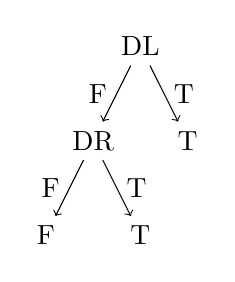
\begin{tikzpicture}[scale=0.8]
  \node (DL) {DL}
    child[->] {
      node (DR) {DR}
        child[->] {node (DRF) {F} edge from parent node[left] {F}}
        child[->] {node (DRT) {T} edge from parent node[right] {T}}
      edge from parent node[left] {F}
    }
    child[->] {node (DLT) {T} edge from parent node[right] {T}};
\end{tikzpicture}

%           DL
%        F / \ T
%         /   \
%        DR    T
%     F / \ T
%      /   \
%     F     T

}
\subfigure[$DL \ \andthen{} \ DR$]{
\label{subfig:DL-and-DR}
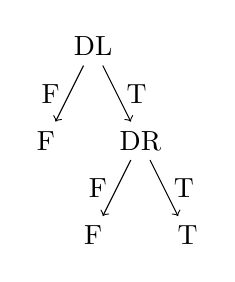
\begin{tikzpicture}[scale=0.8]
  \node (DL) {DL}
    child[->] {node (DLF) {F} edge from parent node[left] {F}}
    child[->] {
      node (DR) {DR}
        child[->] {node (DRF) {F} edge from parent node[left] {F}}
        child[->] {node (DRT) {T} edge from parent node[right] {T}}
      edge from parent node[right] {T}
    };
\end{tikzpicture}

%           DL
%        F / \ T
%         /   \
%        F     DR
%           F / \ T
%            /   \
%           F     T

}
\caption{case 2 and 3}
\end{figure}

There is a diamond in a BDD if and only if there is at least one node
such that the number of paths to reach it from root is strictly
greater than 1; we will use this caracterization to prove our
property.

\emph{Proof of the simplified case:}

Consider first the case where decision D does not contain any negation.
Each node in the BDD corresponds to a sub-decision D' in D
(i.e. the root of each sub-decision is a node in D's BDD).

\emph{Proof of reverse implication (simplified case):}

Let's call NF(D) the number of paths from the root of decision D to False (F)
and NT(D) the number of paths from the root of decision D to True (T). We
then have three cases:

\emph{case 1:} D = A (atom)\\
$NF(D) = NT(D) = 1$

\emph{case 2:} D = $DL \ \orelse{} \ DR$\\
BDD(D) is constructed from BDD(DL) and BDD(DR). It is shown 
in Figure~\ref{subfig:DL-or-DR}. Then:\\
$NF(D) = NF(DL) * NF(DR)$\\
$NT(D) = NT(DL) + NF(DL) * NT(DR)$

\emph{case 3:} D = $DL \ \andthen{} \ DR$\\
BDD(D) is constructed from BDD(DL) and BDD(DR). It is shown 
in Figure~\ref{subfig:DL-and-DR}. Then:\\
$NF(D) = NF(DL) + NT(DL) * NF(DR)$\\
$NT(D) = NT(DL) * NT(DR)$

\begin{lemma}
\label{lemma:NF-NT-bound}
For every decision D, $NF(D) \ge 1$ and $NT(D) \ge 1$.\\
If D is of the form \orelse{} then $NT(D) \ge 2$.\\
If D is of the form \andthen{} then $NF(D) \ge 2$.
\end{lemma}

\begin{lemma}
\label{lemma:NF-NT-monotonic}
NF and NT are monotonic functions, i.e. if D' is a sub-decision of D,
then we have
        $NF(D') \le NF(D)$
and        
        $NT(D') \le NT(D)$.
\end{lemma}

Proofs of Lemmas~\ref{lemma:NF-NT-bound} and~\ref{lemma:NF-NT-monotonic} are on
structural induction on the form of decisions, based on the three cases
distinguished above.

Then, suppose that a decision D of the form \andthen{} contains a
sub-decision D' of the form \orelse{} on the left-hand side. If DL, DR
are the two sub-decisions such that $D = DL \ \andthen{} \ DR$, then D' is
also a sub-decision of DL.

By Lemma~\ref{lemma:NF-NT-bound}, we know that $NT(D') \ge 2$. By
Lemma~\ref{lemma:NF-NT-monotonic}, we know that $NT(DL) \ge NT(D')$.

Then, in BDD(D), the paths reaching the DR's root node are exactly
those paths in BDD(DL) reaching True, by construction; the number of
these paths is NT(DL).

Thus, DR's root node in the BDD(DL) is reachable by more than one
path. As a consequence, there is a diamond in this BDD.

Similarly, if a decision D of the form \orelse{} contains a
sub-decision D' of the form \andthen{} on the left-hand side, we can
exhibit a node in the BDD(D) that is reachable by more
than one path.

By contraposition, if there are no diamonds in the BDD associated to a
decision D, then D has no \orelse{} sub-decision on the left of its
\andthen{} sub-decisions, and no \andthen{} sub-decision to the left of
its \orelse{} sub-decision.

\emph{Proof of implication (simplified case):}

Now suppose that for every sub-decision in decision D, the left
operand of an \andthen{} sub-decision contains only \andthen{}
sub-decisions and the left operand of an \orelse{} sub-decision
contains only \orelse{} sub-decisions.

\begin{lemma}
\label{lemma:NF-NT-only-one-oper}
If E contains only \orelse{} sub-decisions then $NF(E) = 1$.
If E contains only \andthen{} sub-decisions then $NT(E) = 1$.
\end{lemma}

Proof of Lemma~\ref{lemma:NF-NT-only-one-oper} is on structural induction on
the form of decisions, based on the 3 cases distinguished above.

By structural induction on the depth of the BDD, we can show that there cannot
be any diamonds in the BDD associated to D, which proves that the desired
implication holds.

\emph{Proof of the general case:}

In the general case, decision D may contain \adanot{} sub-decisions. Then,
consider D' the negation normal form of D. Since D and D' are represented
by the same BDD, Theorem~\ref{thm:lhs-same-operator} follows.


\section{Coupled conditions}

Handling of coupled conditions is a well-known problem that one has
to face when considering MC/DC, and in particular Unique Cause. It may
be stated as follow:

\begin{definition}
  \label{def:coupled-conditions}
  Two or more conditions are said to be coupled if changing one condition
  can cause the other condition(s) to change.

  Conditions are said to be strongly coupled if changing one always
  changes the others. At the contrary, they are said to be weakly
  coupled if changing one sometimes (but not always) changes the others.
\end{definition}

In \cite{rcdc-from}, it is proved that strongly coupled conditions
are pairs of conditions that are either equal, or complimentary.
In other words, if A and B are strongly coupled, then either $A = B$
or $A = \adanot{} \ B$

Without short-circuit operators, decisions with coupling cannot be
covered for Unique Cause MC/DC; Masking MC/DC has been defined to
solve this problem.  When proving Masking MC/DC for a condition C, one
may exhibit a pair of evaluation that have different values for other
conditions, as long as it can be shown, by a structural analysis of
the decision, that changing these other conditions had no influence
on the result. Typically, for a decision $A \ \adaand{} \ SUBDEC$ ($SUBDEC$
being a sub-decision, $A$ being a condition), any evaluation that sets
$SUBDEC$ to True ensures that only the value of A impacts the value of the
decision. e.g. if $SUBDEC ::= (B \ \adaor{} \ C)$, the following evaluation
pairs proves Masking MC/DC, but not Unique Cause MC/DC:

\begin{center}
\begin{tabular}{|c|c|c||c||c|}
\hline
A & B & C & SUBDEC ::= B \adaor{} C & A \adaand{} SUBDEC \\ \hline
T & F & T & T                       & T \\ \hline
F & T & F & T                       & F \\ \hline
\end{tabular}
\end{center}

B and C change, so Unique Cause MC/DC is not reached; but SUBDEC is kept
to True, so Masking MC/DC is reached. So if C and A were strongly
coupled ($A = C$), we would still be able to cover this decision for Masking
MC/DC; but we would not be able to reach Unique Cause.

When using only short-circuit operators, one may wonder if the problem
still holds. It can be seen that the previous example is covered for Unique
Cause MC/DC when the operators are short-circuit; in this case, the
evaluations are:

\begin{center}
\begin{tabular}{|c|c|c||c||c|}
\hline
A & B & C & A \andthen{} (B \orelse{} C) \\ \hline
T & F & T & T \\ \hline
F & x & x & F \\ \hline
\end{tabular}
\end{center}

So there are some cases of coupling that are not problematic in the case
of short-circuit operator; short-circuits seem to offer some sort of masking
by avoiding to evaluate some sub-decisions. The question would now be:
can we show some cases of coupling for which Unique Cause may not be reached
even with short-circuit operators? Would these cases show up in real life,
or would they be dummy decisions that may be trivially simplified (e.g.
$A \ \andthen{} \ A$)?

The following sections sched some light on these problems. First,
Masking MC/DC is characterized in terms of BDD, in order to make use
of the results that have been demonstrated in the previous sections.
This characterization would then allow to comment on coupling in the
context of short-circuit operators.

\subsection{MC/DC in terms of BDD}

\subsubsection{Unique Cause MC/DC}

\begin{theorem}
  \label{thm:unique-cause-bdd}
  Given a decision D, a pair of evaluations of D satisfies
  Unique Cause MC/DC for a condition C if and only if:
  \begin{itemize}
  \item both reach C using the same path through BDD(D);
  \item their paths from C exits on two different outcomes and do not cross
  each other (C excluded).
  \end{itemize}
\end{theorem}

Let us first prove that this characterization implies Unique Cause MC/DC
as defined previously.

Both evaluations reach C using the same path; this implies that all
conditions that are before C are either not evaluated by any of the
two evaluations, or that they have the same value.  In both cases,
they are colored with False in the influence tree.

After C, their paths through the BDD do not cross each other; this means
that they evaluate C to both values, otherwise they would have at least one
edge in common. C is evaluated to True and False, which means that it is
colored with True in the influence tree.

An other consequence of this hypothesis is that all conditions after C
are not evaluated in at least one of the two paths; a condition that
would be evaluated on both paths would be a meeting point of the two
paths, which would contradict the hypothesis. This means that any
condition after C is colored with False as, by definition, anything
xor Not\_Evaluated gives False.

So, of all conditions, only C is colored with True. As the two
paths exits on two different outcomes, the root node of the influence
tree is colored with True as well. We now have these general properties
of influence trees:

\begin{lemma}
  \label{lemma:influence-tree-props}
  If the root node of an influence tree is colored with True, then
  its influence set is not empty.

  If the root node of an influence tree is colored with True, and
  if only one condition c is colored with True, then the corresponding
  influence set is \{c\}
\end{lemma}

This lemma can be proved by induction on the structure of a decision;
the first property is easier to prove and comes in handy to prove the
second property. We will not detail these proofs here as they offer no
technical difficulty.

Applying the second property to our case, we can now prove that the
influence set of our decision is the singleton \{C\} ; so the two
evaluations satisfy Masking MC/DC. As all other conditions are colored
with False in the influence tree, Unique Cause MC/DC is satisfied.

To demonstrate the other side of the equivalence, let us assume that
one of the two properties on the BDD is violated and let us show that
Unique Cause MC/DC cannot be achieved.

If the two paths are not identical before the considered condition:
they start from the same node (the root of the BDD) and ends up on
the same node (C), so it means that there exists at least one node
from which those paths diverge (this is a general property of paths
through graphs). This node takes therefore two different values
in the two evaluations; so it is colored with True in the influence
tree. It is the second condition colored with True in the influence
tree (with C), so Unique Cause MC/DC cannot be achieved.

If the paths from C cross each other, then there is at least one
condition after C that is evaluated in both paths. Let us call lc the
last condition where the two paths cross. By definition of lc, the two
sub-paths that start from lc and go to outcomes do not cross each
other. This means that they exit by two different edges from lc;
otherwise, the node that they would reach would be a common node after lc,
which would contradict the fact that lc is the last common node. So
lc takes two different values, True and False, on these two paths.
As a consequence, lc is colored with True in the Influence Tree, and
therefore C is not the only one colored with True, so Unique Cause MC/DC
cannot be achieved.

The two sides of the equivalence in Theorem~\ref{thm:unique-cause-bdd}
are now proved.

\subsubsection{Masking MC/DC}

\begin{theorem}
  \label{thm:masking-bdd}
  Given a decision D, a pair of evaluations of D satisfies
  Masking MC/DC for a condition C if and only if:
  \begin{itemize}
  \item both reach C;
  \item their paths from C exit on two different outcomes and do not cross
  each other (C excluded).
  \end{itemize}
\end{theorem}

The difference with Unique Cause is that the paths to reach C may be
different. That is to say: only the sub-bdd of BDD(D) whose root is C
is taken into account when proving Masking MC/DC; anything before C
does not matter (as long as C is reached). An other way to see that:
Masking MC/DC is achieved for C if Unique Cause MC/DC is achieved on
the sub-bdd of BDD(D) whose root is C. Or: any condition on the left
of C is not considered when trying to achieve Masking MC/DC for C.

This may be justified as follow: we have seen that short-circuit operators
do provide some sort of masking in our original example
$A \ \andthen{} \ SUBDEC$. Now, consider $SUBDEC \ \andthen{} \ A$; in this
case, SUBDEC will always be executed before A, so the short-circuit operator
\andthen{} will not mask SUBDEC. Short-circuit operators are non-commutative,
and introduce this asymetricity. Say, if $SUBDEC ::= B \ \orelse \ C$, then
the following evaluations satisfy Masking MC/DC for C, but not Unique Cause:

\begin{center}
\begin{tabular}{|c|c|c||c||c|}
\hline
A & B & C & SUBDEC ::= B \orelse{} C & SUBDEC \andthen{} A \\ \hline
T & F & T & T                        & T \\ \hline
F & T & x & T                        & F \\ \hline
\end{tabular}
\end{center}

For Masking MC/DC, we have to ignore the details of the evaluation of SUBDEC,
as long as it ends up being evaluated to True. In terms of BDD, that means
that we do not care about how we reached the considered condition, as long
as we reached it.

A formal model of this characterisation can be found in
\alloyspec{bdd\_coverage.als}, and a proof of equivalence in a small scope
(at most 4 conditions per decisions) in \alloyspec{bdd\_dec\_coverage.als}.

Here is a proof in the general case. Yet another way to see
Theorem~\ref{thm:masking-bdd} is: a pair of evaluations proves Masking
MC/DC for a condition C if and only if C is the last node where the
two paths to (different) outcomes crosses each other and
diverges. Nodes where these two paths diverges are exactly the
conditions colored with True in the influence tree; and the last node
is the righmost condition.  This means that
Theorem~\ref{thm:masking-bdd} is directly implied by
Lemma~\ref{lemma:short-circuit-influence-set}.

Let us now comment a bit about coupling:
\begin{itemize}

\item We have seen that the only difference between Unique Cause and
Masking MC/DC is the constraint on the way to reach the considered
condition: the same path for both evaluations for Unique Cause, any
path for Masking MC/DC. In a BDD, the path to reach a node is unique
in the case of no diamond; that shall encourage us to have a closer
look at this special case.

\item When we commented about Masking MC/DC, we saw that the
asymetricity of short-circuit was the problem: when two conditions are
coupled, the leftmost one can take advantage of the partial masking that
short-circuit operators provide; however, the rightmost cannot. Now,
can we any problematic case for this rightmost condition? This will be
discussed in the following sections.
\end{itemize}


\subsection{Coupled conditions without diamonds}

First, it can be seen that strong coupling only gives degredated cases,
where some branches of the BDD cannot possibly be covered; this is
what the following theorem states:

\begin{theorem}
  \label{thm:strong-coupling-no-diamond}
  A BDD with no diamonds and with strongly coupled conditions cannot be
  covered for BDD branch coverage, Masking MC/DC, Unique Cause MC/DC.
\end{theorem}

As Unique Cause MC/DC and Masking MC/DC are stronger than BDD branch
coverage, we only need to prove this theorem for BDD branch coverage.

In a BDD with no diamonds, there is only one possible path to each
node, traversing all the previous conditions in the BDD ordering. Take
two strongly coupled conditions; let us call fc the first one in the
BDD ordering, lc the second one. When lc is executed, fc has been
evaluated to a given value, and this value is the same for any
evaluation that reaches lc. Let us call this value $V$. Now, as lc and
fc are strongly coupled, there are only two possibilities: either lc
is always equal to fc, and evaluates to $V$, in which case the exit edge
for $\adanot{} \ V$ is never executed; or it is always the
complementary of c, and evaluates to $\adanot{} \ V$, in which case
the other exit edge is never executed. In any case, BDD branch
coverage cannot be achieved, as at least one edge is never taken.

This means that there are no meaningful cases of strong coupling
without diamonds. They could typically be optimizied out by the
compiler.

We can however exhibit some cases of weak coupling that makes sense.
For instance:

$Dec ::= t > T \ \orelse{} \ (t = T \ \andthen{} \ A)$

Or an even more common pattern, that can often be found in C:

\verb|name != NULL && strcmp (name, "something")|

In these two examples, BDD branch coverage can be reached. For the first
one, it can be checked that these evaluations cover the decision for
BDD branch coverage, Masking MC/DC and Unique Cause MC/DC:

\begin{center}
\begin{tabular}{|c|c|c||c|}
\hline
t > T & t = T & A & Dec \\ \hline
T     & x     & x & T \\ \hline
F     & F     & x & F \\ \hline
F     & T     & T & T \\ \hline
F     & T     & F & F \\ \hline
\end{tabular}
\end{center}

It can be seen that Unique Cause MC/DC and Masking
MC/DC are equivalent in the case of no diamonds, as there is only one
possible path to each node; this is a consequence of
Theorem~\ref{thm:masking-bdd} and Theorem~\ref{thm:unique-cause-bdd}.
So, with no diamonds, Masking MC/DC does not gain us anything, comparing
to Unique Cause MC/DC (or BDD branch coverage):
\begin{itemize}
\item in the cases of strong coupling, none of these coverage criteria
can be reached;
\item in all other cases, all of them are equivalent anyway.
\end{itemize}

If Masking MC/DC is of some help to handle coupled conditions, it has to
be when the decision's BDD contains diamonds. That is the second case that
we will investigate.

\subsection{Coupled conditions with diamonds}

The Theorem~\ref{thm:strong-coupling-no-diamond} cannot be extended to the
case of diamonds. Take for instance this decision:

$Dec ::= (A \ \andthen{} \ B) \ \orelse{} \ (\adanot{} \ A \ \andthen{} \ C)$

This decision is a common pattern, logically equivalent to
$\adaif{} \ A \ \adathen{} \ B \ \adaelse \ C$. It cannot be covered for
Unique Cause MC/DC, because the first and the third condition are strongly
coupled; but it can be covered for Masking MC/DC, with the following
evaluations:

\begin{center}
\begin{tabular}{|c|c|c|c||c|}
\hline
A & B & \adanot{} A & C & Dec\\ \hline
F & x & T           & T & T \\ \hline
F & x & T           & F & F \\ \hline
T & T & x           & x & T \\ \hline
T & F & F           & x & F \\ \hline
\end{tabular}
\end{center}

More precisely: the third condition cannot be covered for Unique Cause;
but the first and the last evaluation cover it for Masking MC/DC.

Another example with weak coupling:

$Dec ::= (t < T \ \andthen{} \ A)
  \ \orelse{} \ (t = T \andthen{} \ B)
  \ \orelse{} \ (t > T \ \andthen{} \ C)$

...which is another case where the logical space is partioned (into three
cases here: $t < T$, $t = T$, $t > T$) using conditions that are such
that exactly one is True for each evaluation.

From the truth table, the only condition for which we cannot reach
Unique Cause is $t > T$:
\begin{itemize}
\item when it is True, both $t < T$ and $t = T$ have been evaluated to False;
\item when it is False, either $t < T$ or $t = T$ has been evaluated to True;
\end{itemize}
so we cannot reach Unique Cause for this one. We can cover it for
Masking MC/DC though, with any of the pairs (eT, eF1) and
(eT, eF2), these three evaluations being:
\begin{itemize}
\item eT = \\
($t < T$ = False, A = Not\_Evaluated,\\
 $t = T$ = False, B = Not\_Evaluated,\\
 $t > T$ = True,  C = True)

\item eF1 = \\
($t < T$ = True,  A = False,\\
 $t = T$ = False, B = Not\_Evaluated,\\
 $t > T$ = False, C = Not\_Evaluated)

\item eF2 = \\
($t < T$ = False, A = Not\_Evaluated,\\
 $t = T$ = True,  B = False,\\
 $t > T$ = False, C = Not\_Evaluated)
\end{itemize}

One could object that this decision may be rewritten as follow:

$(A \ \andthen{} \ t < T)
  \ \orelse{} \ (B \ \andthen{} \ t = T)
  \ \orelse{} \ (C \ \andthen{} \ t > T)$

...in which case Unique Cause MC/DC could be achieved. However, such a
rewriting may not be possible; the execution of condition may have the
precondition that $t < T$, in which case the rewriting would not be
valid. So re-ordering the decision to allow Unique Cause MC/DC to be
reached is not an appropriate general solution to the coupling
problem.

In other words, Masking MC/DC is still useful in the case of
short-circuit operators; but only when there are diamonds in the
decision's BDD.

\newpage
\bibliographystyle{alpha}
\bibliography{references}

\end{document}
